We will now define semigroupoids, which are generalizations of both semigroups and categories. Every category $\mathcal{C}$ comes with an underlying graph structure, where vertices and arrows correspond respectively to objects and morphisms of $\mathcal{C}$. However, the vertex set of $\mathcal{C}$ can always be recovered from the arrow set, by identifying each object to its corresponding identity morphism, and so categories may be defined purely in terms of their arrow space. This becomes an issue in the case of semigroupoids, where we do not have identity elements (or something similar) anymore. We have two working definitions of semigroupoids: One purely algebraic, introduced by Exel in \cite{MR2754831}, and one where we assume an underlying graph structure, introduced by Tilson in \cite{MR915990}. It should be noted that every semigroupoid in the sense of Tilson is a semigroupoid in the sense of Exel (Proposition \ref{prop:graphedsemigroupoidsaresemigroupoids}).

To avoid any confusion, we will use capital greek letters $\Lambda,\Gamma,\ldots$ to denote semigroupoids in the sense of Exel, without a priori underlying graph structures. These are called simply \emph{semigroupoids}, or \emph{Exel semigroupoids} whenever such precision is warranted. Capital caligraphic latin letters $\mathcal{S},\mathcal{T},\ldots$ will be used to denote semigroupoids in the sense of Tilson, with an underlying graph structure, and these will always be called \emph{graphed semigroupoids}.

\begin{definition}[{\cite[Definition 2.1]{MR2754831}}]\label{def:semigroupoid}
An \emph{Exel semigroupoid} or simply \emph{semigroupoid} is a set $\Lambda$ equipped with a subset $\Lambda^{[2]}\subseteq\Lambda\times\Lambda$ and a \emph{product} map $\mu\colon\Lambda^{[2]}\to\Lambda$, denoted by concatenation, $\mu(f,g)=fg$, which is associative in the following sense: For all $f,g,h\in\Lambda$, the statements
\begin{enumerate}[label=(\roman*)]
    \item\label{def:semigroupoiditem1} $(f,g)\in\Lambda^{[2]}$ and $(g,h)\in\Lambda^{[2]}$;
    \item\label{def:semigroupoiditem2} $(f,g)\in\Lambda^{[2]}$ and $(fg,h)\in\Lambda^{[2]}$;
    \item\label{def:semigroupoiditem3} $(g,h)\in\Lambda^{[2]}$ and $(f,gh)\in\Lambda^{[2]}$;
\end{enumerate}
are equivalent and in case any (all) of them holds, we have $(fg)h=f(gh)$. If necessary for precision, we will say instead that the triple $(\Lambda,\Lambda^{[2]},\mu)$ is a semigroupoid.
\end{definition}

We use square brackets when denoting the subset $\Lambda^{[2]}$ of $\Lambda\times\Lambda$ to stress the fact that $\Lambda$ has no graph structure. Moreover, instead of saying that a pair $(f,g)$ belongs to $\Lambda^{[2]}$ we may simply state that ``the product $fg$ is (well-)defined''.

The product of subsets of a semigroupoid $\Lambda$ is regarded in the standard manner: If $A,B\subseteq\Lambda$, the set $AB$ consists of all products $ab$ which are defined, where $a\in A$ and $b\in B$ - that is, $AB=\mu((A\times B)\cap\Lambda^{[2]})$. If $a\in\Lambda$, the products $aA$ and $Aa$ are defined similarly.

The associativity condition on the product may be regarded as follows: if any of the products $(fg)h$ or $f(gh)$ are defined, then the other product is also defined and they are equal, so we simply denote it $fgh$. Also, if $fg$ and $gh$ are both defined, $fgh$ is also defined. This allows us to move parentheses at will during computations.

\begin{example}
Let $\theta$ be a left action of a group $G$ on a set $X$. Consider the disjoint union $\Lambda\defeq G\sqcup X$. We make $\Lambda$ into a semigroupoid by extending the product of $G$ to a partial product on $\Lambda$ with the action, viz.\ $gx=\theta_g(x)$ for all $g\in G$ and $x\in X$.

This is an alternative to the more useful construction of a \emph{transformation groupoid}, which is a particular case of a semidirect product of semigroupoids (see Subection \ref{sec:dualprehomomorphisms}).
\end{example}

Let us look at some counter-examples for the associativity condition, where some of items \ref{def:semigroupoiditem1}-\ref{def:semigroupoiditem3} are valid but the others are not.

\begin{example}
Let $\Lambda=\left\{f,g,h\right\}$, and define $fg=f$ and $gh=h$. Then $fg$ and $gh$ are defined, but neither $(fg)h$ nor $f(gh)$ are defined.
\end{example}

\begin{example}
Let $\Lambda=\left\{f,g,h\right\}$, and define $fg=g$, $gh=h$. Then $fg$, $gh$ and $(fg)h$ are defined, but $f(gh)$ is not. A similar example may be constructed, where $f(gh)$ is defined but $(fg)h$ is not.
\end{example}

\begin{example}
Let $\Lambda=\left\{f,g,h\right\}$ with product $fg=hh=h$. Then $(fg)h$ is defined, but $gh$ is not. A similar example may be constructed where $f(gh)$ is defined but $fg$ is not.
\end{example}

\begin{example}
If $\Lambda$ is any set endowed with a non-associative binary operation, then \ref{def:semigroupoiditem1}-\ref{def:semigroupoiditem3} of Definition \ref{def:semigroupoid} are always valid, and in particular equivalent, but $\Lambda$ is not a semigroupoid. For example, take $\Lambda=\left\{a,b\right\}$, $aa=ab=b$, $bb=ba=a$. Then $(aa)a=a$ but $a(aa)=b$.
\end{example}

Sub-semigroupoids and semigroupoid homomorphisms are defined in the natural manner.

\begin{definition}
A \emph{sub-semigroupoid} of a semigroupoid $\Lambda$ is a subset $\Delta\subseteq\Lambda$ such that $\Delta\Delta\subseteq\Delta$.
\end{definition}

\begin{definition}
A \emph{homomorphism} between semigroupoids $\Lambda$ and $\Gamma$ is a map $\phi\colon\Lambda\to\Gamma$ such that $(\phi\times\phi)(\Lambda^{[2]})\subseteq\Gamma^{[2]}$ and $\phi(ab)=\phi(a)\phi(b)$ for all $(a,b)\in\Lambda^{[2]}$.
\end{definition}

It is immediate to verify that if $\phi\colon \Lambda\to\Gamma$ is a homomorphism of semigroupoids and $\Delta$ is a sub-semigroupoid of $\Gamma$, then $\phi^{-1}(\Delta)$ is a sub-semigroupoid of $\Lambda$. However, contrary to the cases of semigroups and groupoids, the image of a homomorphism $\phi\colon\Lambda\to\Gamma$ between semigroupoids is not necessarily a sub-semigroupoid of $\Gamma$.

\begin{example}\label{ex:imageofhomomorphismisnotasubsemigroupoid}
    Let $\Lambda=\left\{e,f\right\}$, with operations $ee=e$ and $ff=f$ and $\Gamma=\left\{e,f,g\right\}$ the semigroup with product $ee=e$, $ff=f$, and all other products $xy=g$. Then the inclusion $\iota\colon\Lambda\hookrightarrow\Gamma$ is a semigroupoid homomorphism, but the image $\iota(\Lambda)=\left\{e,f\right\}$ is not sub-semigroupoid of $\Gamma$.
\end{example}

We will now consider semigroupoids in the sense of Tilson.

\begin{definition}[{\cite[p.\ 194]{MR915990}}]\label{def:graphedsemigroupoid}
A \emph{graphed semigroupoid} is a tuple $(\mathcal{S}^{(0)},\mathcal{S},\so,\ra,\mu)$, where $(\mathcal{S}^{(0)},\mathcal{S},\so,\ra)$ is a graph and $\mu\colon\mathcal{S}^{(2)}\to\mathcal{S}$ is a \emph{product map}, denoted by concatenation, $\mu(a,b)=ab$, satisfying:
\begin{enumerate}[label=(\roman*)]
    \item\label{def:graphedsemigroupoiditem1} for all $(a,b)\in \mathcal{S}^{(2)}$, $\so(ab)=\so(b)$ and $\ra(ab)=\ra(a)$ -- i.e., $(\id_{\mathcal{S}^{(0)}},\mu)$ is a graph morphism;
    \item\label{def:graphedsemigroupoiditem2} for all $(a,b,c)\in \mathcal{S}^{(3)}$, $(ab)c=a(bc)$.
\end{enumerate}
We will always assume that a graphed semigroupoid $\mathcal{S}$ satisfies $\mathcal{S}^{(0)}=\so(\mathcal{S})\cup\ra(\mathcal{S})$. Otherwise, restricting the vertex set to $\so(\mathcal{S})\cup\ra(\mathcal{S})$ yields another graphed semigroupoid with the same underlying arrow set and product.
\end{definition}

The next proposition shows that graphed semigroupoids are, in particular, Exel semigroupoids.

\begin{proposition}\label{prop:graphedsemigroupoidsaresemigroupoids}
Let $(\mathcal{S}^{(0)},\mathcal{S},\so,\ra)$ be a graph and $\mu\colon\mathcal{S}^{(2)}\to \mathcal{S}$, $\mu(a,b)=ab$, a fixed function. Consider the following assertions:
\begin{enumerate}[label=(\arabic*)]
    \item\label{prop:graphedsemigroupoidsaresemigroupoidsitem1} $(\mathcal{S}^{(0)},\mathcal{S},\so,\ra,\mu)$ is a graphed semigroupoid;
    \item\label{prop:graphedsemigroupoidsaresemigroupoidsitem2} $(\mathcal{S},\mathcal{S}^{(2)},\mu)$ is an Exel semigroupoid.
    \item\label{prop:graphedsemigroupoidsaresemigroupoidsitem3} for all $(a,b)\in \mathcal{S}^{(2)}$, $\so(ab)=\so(b)$ and $\ra(ab)=\ra(b)$.
\end{enumerate}
Then \ref{prop:graphedsemigroupoidsaresemigroupoidsitem1} is equivalent to \ref{prop:graphedsemigroupoidsaresemigroupoidsitem2}+\ref{prop:graphedsemigroupoidsaresemigroupoidsitem3} (that is, their logical conjunction).

If $\mathcal{S}$ has no sources nor sinks, then \ref{prop:graphedsemigroupoidsaresemigroupoidsitem2} implies \ref{prop:graphedsemigroupoidsaresemigroupoidsitem3}. (Thus \ref{prop:graphedsemigroupoidsaresemigroupoidsitem1} is equivalent to \ref{prop:graphedsemigroupoidsaresemigroupoidsitem2} in this case.)
\end{proposition}
\begin{proof}
    The implication \ref{prop:graphedsemigroupoidsaresemigroupoidsitem2}+\ref{prop:graphedsemigroupoidsaresemigroupoidsitem3}$\Rightarrow$\ref{prop:graphedsemigroupoidsaresemigroupoidsitem1} is trivial.
    
    The only nontrivial part of the implication \ref{prop:graphedsemigroupoidsaresemigroupoidsitem1}$\Rightarrow$\ref{prop:graphedsemigroupoidsaresemigroupoidsitem2}+\ref{prop:graphedsemigroupoidsaresemigroupoidsitem3} is the verification that items \ref{def:semigroupoiditem1}-\ref{def:semigroupoiditem3} of Definition \ref{def:semigroupoid} are equivalent: In other words, to compare when products $ab$, $bc$, $a(bc)$ and $(ab)c$ are defined.
    
    For example, assume that \ref{def:semigroupoid}\ref{def:semigroupoiditem1} is valid, i.e., $(a,b)\in\mathcal{S
    }^{(2)}$ and $(b,c)\in\mathcal{S
    }^{(2)}$. Then $\so(ab)=\so(b)=\ra(c)$, so $(ab,c)\in\mathcal{S
    }^{(2)}$, which means that \ref{def:semigroupoid}\ref{def:semigroupoiditem2} is valid. The other implications are proven similarly. Therefore \ref{prop:graphedsemigroupoidsaresemigroupoidsitem1} implies \ref{prop:graphedsemigroupoidsaresemigroupoidsitem2}+\ref{prop:graphedsemigroupoidsaresemigroupoidsitem3}.
    
    For the last part, assume that $(\mathcal{S
    },\mathcal{S
    }^{(2)},\mu)$ is an Exel semigroupoid and that the graph $\mathcal{S
    }$ has no sources nor sinks, and let us verify \ref{prop:graphedsemigroupoidsaresemigroupoidsitem3}. Let $(a,b)\in\mathcal{S
    }^{(2)}$. As the vertex $\so(b)$ is not a source of $\mathcal{S
    }$, choose $z\in\mathcal{S
    }$ such that $(b,z)\in\mathcal{S
    }^{(2)}$. Then $(ab,z)\in\mathcal{S
    }^{(2)}$, because $(\mathcal{S
    },\mathcal{S
    }^{(2)},\mu)$ is an Exel semigroupoid, which means that $\so(ab)=\ra(z)=\so(b)$. Similarly, $\mathcal{S
    }$ not having sinks implies that $\ra(ab)=\ra(a)$. This is precisely property \ref{prop:graphedsemigroupoidsaresemigroupoidsitem3}.\qedhere
\end{proof}

\begin{example}
Every semigroup $S$ may be regarded as a graphed semigroupoid with a singleton vertex set, $S^{(0)}=\left\{\ast\right\}$. Conversely, every graphed semigroupoid (or rather its arrow set) with singleton vertex set is a semigroup.
\end{example}

We will now characterize Exel semigroupoids which admit a compatible graph structure (Proposition \ref{prop:equivalencegraphableandcategoricalsemigroupoids}). These were already considered in \cite{MR2419901}. We will moreover classify all compatible graph structures to such an Exel semigroupoid (Proposition \ref{prop:classificationofgraphsoncategorical}).

\begin{definition}[{\cite[Definition 19.1]{MR2419901}}]
Let $\Lambda$ be an Exel semigroupoid. For every $a\in\Lambda$, we define
\[\Lambda^a=\left\{b\in\Lambda:(a,b)\in\Lambda^{[2]}\right\},\qquad\Lambda_a=\left\{b\in\Lambda:(b,a)\in\Lambda^{[2]}\right\}.\]
We say that $\Lambda$ is \emph{categorical} if for all $a,b\in\Lambda$, the sets $\Lambda^a$ and $\Lambda^b$ are either disjoint or equal.
\end{definition}

Note that $b\in\Lambda^a$ if and only if $a\in\Lambda_b$. Moreover, $\Lambda^{ab}=\Lambda^b$ and $\Lambda_{ab}=\Lambda_a$ for all $(a,b)\in\Lambda^{[2]}$.

\begin{proposition}\label{prop:equivalencecategorical}
The following are equivalent for an Exel semigroupoid $\Lambda$:
\begin{enumerate}[label=(\arabic*)]
  \item\label{prop:equivalencecategoricalitem1} $\Lambda$ is categorical.
  \item\label{prop:equivalencecategoricalitem2} For all $a,b\in\Lambda$, $\Lambda_a$ and $\Lambda_b$ are either disjoint or equal.
\end{enumerate}
\end{proposition}
\begin{proof}
  Assume that $\Lambda$ is categorical and let $a,b\in\Lambda$. We need to prove that if $\Lambda_a$ and $\Lambda_b$ are not disjoint, then they are equal. Suppose $p\in\Lambda_a\cap\Lambda_b$. By symmetry, it is sufficient to prove that $\Lambda_a\subseteq\Lambda_b$.
  
  Given $r\in\Lambda_a$, we have $a\in\Lambda^p\cap\Lambda^r$. Therefore, $\Lambda^p=\Lambda^r$, as $\Lambda$ is categorical. As $b\in\Lambda^p=\Lambda^r$, then $r\in\Lambda_b$. Therefore \ref{prop:equivalencecategoricalitem2} is valid.
  
  The implication \ref{prop:equivalencecategoricalitem2}$\Rightarrow$\ref{prop:equivalencecategoricalitem1} is completely analogous.\qedhere
\end{proof}

We will now prove that categorical semigroupoids are precisely those with a compatible graph structure. All that is needed is to define an appropriate vertex set and source and range maps. The main idea is that if $\mathcal{S}$ is a graphed semigroupoid and $(a,z)\in\mathcal{S
    }^{(2)}$, then for any other arrow $c\in\mathcal{S
    }$, we have $\so(c)=\so(a)$ if and only if $c\in\mathcal{S
    }_z$. This suggests us to identify $\so(a)$ with $\mathcal{S
    }_z$, and this is where the categorical property comes into play. If $\mathcal{S
    }^a=\varnothing$ (i.e., there is no $z$ such that $(a,z)\in\mathcal{S
    }^{(2)}$), then we add a ``dummy'' vertex as the source of $a$.

\begin{theorem}\label{prop:equivalencegraphableandcategoricalsemigroupoids}
Every graphed semigroupoid is categorical. Conversely, every categorical Exel semigroupoid $(\Lambda,\Lambda^{[2]},\mu)$ can be graphed, i.e., we may construct a graphed semigroupoid $(\Lambda^{(0)},\Lambda,\so,\ra,\mu)$, in such a way that $\Lambda^{[2]}=\Lambda^{(2)}$.
\end{theorem}
\begin{proof}
Suppose that $(\mathcal{S
    }^{(0)},\mathcal{S
    },\so,\ra,\mu)$ is a graphed semigroupoid and $a,b\in\mathcal{S
    }$. If $\mathcal{S
    }^a$ and $\mathcal{S
    }^b$ are not disjoint, take any $p\in\mathcal{S
    }^a\cap\mathcal{S
    }^b$. For all $q\in\mathcal{S
    }^a$, we have
\[\ra(q)=\so(a)=\ra(p)=\so(b)\]
thus $q\in\mathcal{S}^b$. This proves $\mathcal{S
    }^a\subseteq\mathcal{S
    }^b$, and the reverse inclusion is proven similarly. Hence $\mathcal{S
    }$ is categorical.

Conversely, assume that $(\Lambda,\Lambda^{[2]},\mu)$ is a categorical semigroupoid. We will first construct the vertex set of the underlying graph of $\Lambda$.

Consider two collections of symbols \[V_0=\left\{v_0(a):a\in\Lambda,\Lambda^a=\varnothing\right\}\qquad\text{and}\qquad V_1=\left\{v_1(a):a\in\Lambda,\Lambda_a=\varnothing\right\}.\]
Let $R_0$ and $R_1$ be any two equivalence relations on $V_0$ and $V_1$, respectively, satisfying, for all $(a,b)\in\Lambda^{[2]}$,
\[\text{if }\Lambda^b=\varnothing\text{ then }(v_0(b),v_0(ab))\in R_0\qquad\text{and}\qquad\text{if }\Lambda_a=\varnothing\text{ then }(v_1(a),v_1(ab))\in R_1.\ntag\label{eq:additionalpropertyofequivalencerelations}\]
We denote the $R_i$-equivalence class of a symbol $v_i(a)\in V_i$ as $[v_i(a)]$ (where $a\in\Lambda)$.

Define the vertex set $\Lambda_{R_0,R_1}^{(0)}$ as the disjoint union $\left\{\Lambda_a:a\in\Lambda,\Lambda_a\neq\varnothing\right\}\sqcup(V_0/R_0)\sqcup(V_1/R_1)$, and the source and range maps $\so_{R_0,R_1},\ra_{R_0,R_1}\colon\Lambda\to\Lambda_{R_0,R_1}^{(0)}$ as
\[\so_{R_0,R_1}(a)=\begin{cases}
\Lambda_z,&\text{if }z\text{ is any element of } \Lambda^a\\
[v_0(a)],&\text{if }\Lambda^a=\varnothing,
\end{cases}\qquad\text{and}\qquad \ra_{R_0,R_1}(a)=\begin{cases}
\Lambda_a,&\text{if }\Lambda_a\neq\varnothing,\\
[v_1(a)],&\text{if }\Lambda_a=\varnothing.
\end{cases}
\]
\[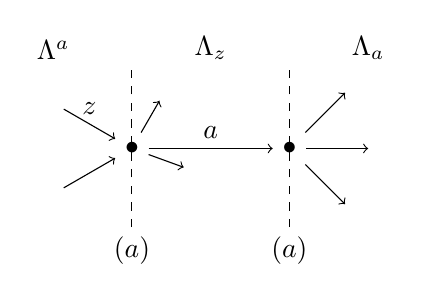
\begin{tikzpicture}
\node (Sa) at (0,0) {$\bullet$};
\node (Ra) at (2,0) {$\bullet$};
\draw[->] (Sa)--(Ra) node[above,align=center,midway] {$a$};
\draw[dashed] (Sa)+(-90:1) node[below] {$\so(a)$} -- +(90:1);
\draw[dashed] (Ra)+(-90:1) node[below] {$\ra(a)$}-- +(90:1);
\draw[->] (Sa)--+(60:0.7);
\draw[->] (Sa)--+(-20:0.7);
\node[above] at (1,1) {$\Lambda_z$};
\draw[->] (Ra) -- +(45:1);
\draw[->] (Ra) -- +(-45:1);
\draw[->] (Ra) -- +(0:1);
\draw[->] (Sa)+(150:1) -- (Sa) node[midway,above] {$z$};
\draw[->] (Sa)+(210:1) -- (Sa);
\node[above] at (3,1) {$\Lambda_a$};
\node[above] at (-1,1) {$\Lambda^a$};
\end{tikzpicture}
\]
We need to check that the source map is well-defined: if $\Lambda^a$ is nonempty and $z_1,z_2\in\Lambda^a$, then $a\in\Lambda_{z_1}\cap\Lambda_{z_2}$, which is therefore nonempty and thus $\Lambda_{z_1}=\Lambda_{z_2}$ because $\Lambda$ is categorical. Moreover, note that if $z\in\Lambda^a$, then $a\in\Lambda_z\neq\varnothing$, so $\Lambda_z\in\Lambda_{R_0,R_1}^{(0)}$.

This defines a graph structure on $\Lambda$. Since it depends on $R_0$ and $R_1$, we denote the set of $2$-paths as $\Lambda_{R_0,R_1}^{(2)}$. We need to prove that $\Lambda^{[2]}=\Lambda_{R_0,R_1}^{(2)}$. 

If $(a,b)\in\Lambda^{[2]}$, then $b\in\Lambda^a$, so $\so(a)=\Lambda_b$. Also, $a\in\Lambda_b$, which is nonempty and thus $\ra(b)=\Lambda_b=\so(a)$. This proves $\Lambda^{[2]}\subseteq\Lambda_{R_0,R_1}^{(2)}$.

Conversely, suppose that $(a,b)\in\Lambda_{R_0,R_1}^{(2)}$, that is, that $\so(a)=\ra(b)$. By the definitions of $\Lambda_{R_0,R_1}^{(2)}$ (as a disjoint union) and of the source and range maps, we necessarily have $\so(a)=\ra(b)\in\left\{\Lambda_z:z\in\Lambda\right\}$, that is, that $\so(a)=\Lambda_z$ for some $z\in\Lambda^a$, and that $\ra(b)=\Lambda_b$. Then
\[a\in\Lambda_z=\so(a)=\ra(b)=\Lambda_b,\]
which means that $(a,b)\in\Lambda^{[2]}$.

Finally, since $\Lambda^{ab}=\Lambda^b$ and $\Lambda_{ab}=\Lambda_a$ for all $(a,b)\in\Lambda^{(2)}$, we obtain $\ra(ab)=\ra(a)$ and $\so(ab)=\so(b)$ (this is where Equation \eqref{eq:additionalpropertyofequivalencerelations} is necessary). By Proposition \ref{prop:graphedsemigroupoidsaresemigroupoids}, $(\Lambda_{R_0,R_1}^{(0)},\Lambda,\so,\ra,\mu)$ is a graphed semigroupoid.\qedhere
\end{proof}

The construction above, in fact, yields \emph{all} the compatible graph structures on $\Lambda$, as we now prove. Let $V_0$ and $V_1$ be the two sets considered in the proof above.

\begin{proposition}\label{prop:classificationofgraphsoncategorical}
Let $\Lambda$ be a categorical Exel semigroupoid, endowed with a graph structure which makes it a graphed semigroupoid $(\Lambda^{(0)},\Lambda,\so,\ra,\mu)$. Suppose, moreover, that $\Lambda^{(0)}=\so(\Lambda)\cup\ra(\Lambda)$.

Then there exist unique equivalence relations $R_0$ and $R_1$ on $V_0$ and $V_1$, respectively, and a bijection $I\colon\Lambda_{R_0,R_1}^{(0)}\to\Lambda^{(0)}$ such that $(I,\id_{\Lambda})$ is a graph isomorphism.
\end{proposition}
\begin{proof}
Consider the sets \[W_0=\left\{\so(a):\Lambda^a=\varnothing\right\},\qquad W_1=\left\{\ra(a):\Lambda_a=\varnothing\right\}\qquad\text{and}\qquad W=\Lambda^{(0)}\setminus(W_0\cup W_1).\]
Note that $W_0$ and $W_1$ are disjoint, since otherwise there would be $a,b\in\Lambda$ such that $\so(a)=\ra(b)$ and $\Lambda_b=\varnothing$. However, this would imply that $(a,b)\in\Lambda^{(2)}$, so $a\in\Lambda_b$, a contradiction.

First we need to construct the equivalence relations $R_0$ and $R_1$ as in Proposition \ref{prop:equivalencegraphableandcategoricalsemigroupoids}. Consider the functions $F_0\colon V_0\to W_0$ and $F_1\colon V_1\to W_1$ given by
\[F_0(v_0(a))=\so(a)\qquad\text{and}\qquad F_1(v_1(b))=\ra(b)\]
for all $a,b\in\Lambda$ such that $\Lambda^a=\Lambda_b=\varnothing$. Note that these maps are surjective. Consider the equivalence relations $R_i=\ker F_i$ ($i=1,2$), that is,
\[R_i=\left\{(v_i(a),v_i(b)):F_i(v_i(a))=F_i(v_i(b))\right\}.\]
Then Equation \eqref{eq:additionalpropertyofequivalencerelations} is clearly satisfied, by the definition of $F_0$ and $F_1$ and because $\so$ and $\ra$ are compatible with the semigroupoid structure of $\Lambda$ (see Definition \ref{def:graphedsemigroupoid}\ref{def:graphedsemigroupoiditem1}).

Therefore the maps $F_i$ factor through the quotient to bijections $V_i/R_i\to W_i$. This gives us a bijection
\[I\colon(V_0/R_0)\sqcup(V_1/R_1)\to W_0\cup W_1,\qquad I([v_i(a)])=F_i(v_i(a)).\]
We need to extend $I$ to a bijection from $\Lambda_{R_0,R_1}^{(0)}$ to $\Lambda^{(0)}$, that is, we need to define $I(\Lambda_a)$ when $\Lambda_a\neq\varnothing$ in order to obtain a bijection from $\left\{\Lambda_a:\Lambda_a\neq\varnothing\right\}$ to $W$.

If $\Lambda_a\neq\varnothing$, we let $I(\Lambda_a)=\ra(a)$. In order to prove that $I$ is well-defined, suppose $\Lambda_{a_1}=\Lambda_{a_2}\neq\varnothing$. Choose any $z\in\Lambda_{a_1}=\Lambda_{a_2}$, so $(z,a_i)\in\Lambda^{(2)}$, that is, $\ra(a_1)=\so(z)=\ra(a_2)$, so $I(\Lambda_a)$ is uniquely defined.

Now let us prove that $I(\Lambda_a)\in W$ whenever $\Lambda_a\neq\varnothing$, or equivalently that $I(\Lambda_a)\not\in W_0\cup W_1$.
\begin{itemize}
    \item If $\ra(a)=\so(b)$ then $a\in\Lambda^b$ and in particular $\Lambda^b\neq\varnothing$. This proves that $I(\Lambda_a)\not\in W_0$;
    \item If $\ra(a)=\ra(b)$, then $\Lambda_a=\Lambda_b$. As $\Lambda_a\neq\varnothing$, this proves that $I(\Lambda_a)\not\in W_1$.
\end{itemize}
Therefore $I(\Lambda_a)\in\Lambda^{(0)}\setminus(W_0\cup W_1)=W$.

Let us now prove that every $v\in W$ is of the form $I(\Lambda_a)$ for some $a\in\Lambda$ with $\Lambda_a\neq\varnothing$. As we assume that $\Lambda^{(0)}=\so(\Lambda)\cup\ra(\Lambda)$, we have two possibilities:
\begin{itemize}
    \item If $v=\so(b)$ for some $b$, then $\Lambda^b\neq\varnothing$, as $v\not\in W_0$, so we may take any $a\in\Lambda^b$. We have $b\in\Lambda_a\neq\varnothing$, and $I(\Lambda_a)=\ra(a)=\so(b)=v$.
    \item If $v=\ra(a)$ for some $a$, then $\Lambda_a\neq\varnothing$ as $v\not\in W_1$, and so $v=I(\Lambda_a)$.
\end{itemize}

We have thus obtained a surjection $I\colon\left\{\Lambda_a:\Lambda_a\neq\varnothing\right\}\to W$. We still need to prove that $I$ is injective on this set. Suppose $I(\Lambda_a)=I(\Lambda_b)$, that is, $\ra(a)=\ra(b)$, where $\Lambda_a,\Lambda_b\neq\varnothing$. Choose any $z\in\Lambda_a$. Then $\so(z)=\ra(a)=\ra(b)$, so $z\in\Lambda_a\cap\Lambda_b$, and therefore $\Lambda_a=\Lambda_b$ as $\Lambda$ is categorical.

We have, therefore, a well-defined bijection $I\colon\Lambda_{R_0,R_1}^{(0)}\to\Lambda^{(0)}$. We are done if we verify that $\so(a)=I(\so_{R_0,R_1}(a))$ and $\ra(a)=I(\ra_{R_0,R_1}(a))$ for all $a\in\Lambda$. Let $a\in\Lambda$. If $\Lambda^a=\varnothing$, then
\[I(\so_{R_0,R_1}(a))=I([v_0(a)])=F_0(v_0(a))=\so(a).\]
If $\Lambda^a\neq\varnothing$, then we choose $z\in\Lambda^a$, so that $a\in\Lambda_z\neq\varnothing$, and
\[I(\so_{R_0,R_1}(a))=I(\Lambda_z)=\ra(z)=\so(a).\]

This proves that $I\circ\so_{R_0,R_1}=\so$, and similarly $I\circ\ra_{R_0,R_1}=\ra$. Therefore $(I,\id_\Lambda)$ is a graph isomorphism.

Suppose now that $R_0'$ and $R_1'$ are any other equivalence relations on $V_0$ and $V_1$ and $J\colon\Lambda_{R_0',R_1'}^{(0)}\to\Lambda^{(0)}$ is any other bijection for which $(J,\id_{\Lambda})$ is a graph isomorphism. We denote the equivalence classes of $V_i/R_i'$ as $[v_i(a)]'$. For each $v_0(a),v_0(b)\in V_0$, where $\Lambda^a=\Lambda^b=\varnothing$, we have
\[\begin{array}{c c c c c}
    v_0(a)R_0'v_0(b)&\iff&[v_0(a)]'=[v_0(b)]'&\iff& J([v_0(a)]')=J([v_0(b)]')\\
    &\iff& J(\so_{R_0',R_1'}(a))=J(\so_{R_0',R_1'}(b))&\iff& \so(a)=\so(b)\\
    &\iff& F_0(v_0(a))=F_0(v_0(b))&\iff& v_0(a)R_0 v_0(b),
\end{array}\]
where we use the facts that $J$ is injective, the definition of the source map $\so_{R_0',R_1'}$, the fact that $(J,\id_{\Lambda})$ is a graph isomorphism, and the definitions of $F_0$ and of $R_0=\ker F_0$. Therefore $R_0'=R_0$. Similarly, $R_1'=R_1$.\qedhere
\end{proof}

\begin{example}
Let $\Lambda=\left\{a,b,x,y,z\right\}$, with product defined by
\[aa=a,\quad xa=y,\quad ya=y,\quad bb=b, \quad xb=z,\quad zb=z\]
Then $\Lambda$ is a non-categorical semigroupoid, since $\Lambda_a=\left\{x,y\right\}$ and $\Lambda_b=\left\{x,z\right\}$ are different but not disjoint. Thus $\Lambda$ cannot be fully realized as a graphed semigroupoid.
\end{example}

Note that every Exel semigroupoid $\Lambda$ may be identified, in an injective and homomorphic manner, as a subset of some semigroup $S$: Namely, the power set $S=2^\Lambda$ of $\Lambda$ is a semigroup under the product of sets, and the map $\phi\colon\Lambda\to S$, $\phi(a)=\left\{a\right\}$, is an injective semigroupoid homomorphisms. However, $\phi(\Lambda)$ is not a sub-semigroup(oid) of $S$ if $\Lambda$ is not a semigroup itself.

We finish this introduction by providing a condition that allows us to ``extend'' semigroupoid homomorphisms between graphed semigroupoids to graph homomorphisms.

\begin{proposition}\label{prop:vertexmap}
Suppose that $G$ and $H$ are graphs, that $G$ has no sources nor sinks, and that $\phi\colon G\to H$ is a map such that $(\phi\times\phi)(G^{(2)})\subseteq H^{(2)}$. Then there exists a unique ``vertex map'' $\phi^{(0)}\colon G^{(0)}\to H^{(0)}$ such that $(\phi^{(0)},\phi)$ is a graph morphism.
\end{proposition}
\begin{proof}
Uniqueness of such $\phi^{(0)}$ is immediate, since we require that $\so_H\circ\phi=\phi^{(0)}\circ\so_G$, and $\so_G$ is surjective as $G$ has no sinks. This same equation yields us the only possible formula for $\phi^{(0)}$, viz.\ $\phi^{(0)}(v)=\so_H(\phi(a))$ where $a\in G$ is any arrow with $\so_G(a)=v$. Thus we need to verify that $\so_G(a)=\so_G(b)$, where $a,b\in G$, implies $\so_H(\phi(a))=\so_H(\phi(b))$. As $\so_G(a)$ is not a source, there exists $z\in G$ with $\ra_G(z)=\so_G(a)=\so_G(b)$, that is $(a,z)$ and $(b,z)\in G^{(2)}$. Then $(\phi(a),\phi(z))$ and $(\phi(b),\phi(z))\in H^{(2)}$, which means that
\[\so_H(\phi(a))=\ra_H(\phi(z))=\so_H(\phi(b)).\]
Therefore, we obtain a unique function $\phi^{(0)}\colon G^{(0)}\to H^{(0)}$ satisfying $\so_H\circ\phi=\phi^{(0)}\circ\so_G$. The proof that $\ra_H\circ\phi=\phi^{(0)}\circ\ra_G$ follows a similar argument as in the paragraph above, but using instead the fact that $G$ has no sinks.\qedhere
\end{proof}

\begin{corollary}\label{cor:graphedhomomorphisminducesvertexmap}
Suppose that $\mathcal{S}$ and $\mathcal{T}$ are graphed semigroupoids, $\phi\colon\mathcal{S}\to\mathcal{T}$ is a semigroupoid homomorphism, and that $\mathcal{S}$ has no sources nor sinks. Then there exists a unique ``vertex map'' $\phi^{(0)}\colon\mathcal{S}^{(0)}\to\mathcal{T}$ such that $(\phi^{(0)},\phi)$ is a graph homomorphism.
\end{corollary}

\begin{example}
The proposition above is not valid if we just assume that $\mathcal{S}$ has no sinks (or no sources). Let us associate a semigroupoid $A$ to the \emph{strict} order of $\mathbb{N}$ in the same manner as we associate categories to (non-strict) orders -- namely $A=\left\{(n,m)\in\mathbb{N}\times\mathbb{N}:m<n\right\}$, with product $(n,m)(m,k)=(n,k)$, vertex set $A^{(0)}=\mathbb{N}$ and source and range maps $\so(n,m)=m$, $\ra(n,m)=n$.

Now let $\mathcal{S}_1=A\sqcup A$ consist of two distinct copies of $A$, so $\mathcal{S}_1$ is a graphed semigroupoid over $\mathcal{S}_1^{(0)}=\mathbb{N}\sqcup\mathbb{N}$ (the product of $\mathcal{S}_1$ is defined only for elements in the same copy of $A$). We let $\mathcal{S}_2^{(0)}$ be the set obtained from $\mathcal{S}_1^{(0)}=\mathbb{N}\sqcup\mathbb{N}$ by identifying both copies of $0$, and let $\mathcal{S}_2$ be the graphed semigroupoid obtained from $\mathcal{S}_1$ by composing the source and range maps with the canonical quotient map $\mathcal{S}_1^{(0)}\to\mathcal{S}_2^{(0)}$.
\[
\begin{tikzpicture}
\node (S2) at (0,0) {$\mathcal{S}_2$:};
\node (S20) at ([shift={+(0.5,0)}]S2) {$0$};
\node (S211) at ([shift={+(1,0.5)}]S20) {$1$};
\node (S212) at ([shift={+(1,-0.5)}]S20) {$1$};
\node (S221) at ([shift={+(1,0)}]S211) {$2$};
\node (S222) at ([shift={+(1,0)}]S212) {$2$};
\node (S231) at ([shift={+(1,0)}]S221) {$\cdots$};
\node (S232) at ([shift={+(1,0)}]S222) {$\cdots$};
\draw[->] (S20)--(S211);
\draw[->] (S211)--(S221);
\draw[->] (S221)--(S231);
\draw[->] (S20)--(S212);
\draw[->] (S212)--(S222);
\draw[->] (S222)--(S232);



\node (S1) at ([shift={+(-6,0)}]S2) {$\mathcal{S}_1$:};
\node (S101) at ([shift={+(0.5,0.5)}]S1) {$0$};
\node (S102) at ([shift={+(0.5,-0.5)}]S1) {$0$};
\node (S111) at ([shift={+(1,0)}]S101) {$1$};
\node (S112) at ([shift={+(1,0)}]S102) {$1$};
\node (S121) at ([shift={+(1,0)}]S111) {$2$};
\node (S122) at ([shift={+(1,0)}]S112) {$2$};
\node (S131) at ([shift={+(1,0)}]S121) {$\cdots$};
\node (S132) at ([shift={+(1,0)}]S122) {$\cdots$};
\draw[->] (S101)--(S111);
\draw[->] (S111)--(S121);
\draw[->] (S121)--(S131);
\draw[->] (S102)--(S112);
\draw[->] (S112)--(S122);
\draw[->] (S122)--(S132);
\end{tikzpicture}
\]
Then neither $\mathcal{S}_1$ nor $\mathcal{S}_2$ have sinks, but the identity map $\mathcal{S}_2\to\mathcal{S}_1$ is an Exel semigroupoid isomorphism which cannot be extended to a graph homomorphism.
\end{example}